\documentclass{article}

\usepackage[english]{babel}
\usepackage[utf8]{inputenc}
\usepackage{amsmath,amssymb}
\usepackage{tabularx}
\usepackage{booktabs}
\usepackage{enumitem}
\usepackage{parskip}
\usepackage{graphicx}

\usepackage[top=2.5cm, left=3cm, right=3cm, bottom=4.0cm]{geometry}

\usepackage{caption}
\usepackage{subcaption}
\usepackage{subfigure}
\usepackage[section]{placeins}
\usepackage{float}
\usepackage{minted}

\usepackage{graphicx}
\usepackage[%  
    colorlinks=true,
    pdfborder={0 0 0},
    linkcolor=blue
]{hyperref}

\newcommand{\lectureheader}[4]{%
  \begin{minipage}{.3\textwidth}%
    
    \strut\includegraphics[scale=1.5]{ethlogo.pdf}%
  \end{minipage} \hfill%
  \raisebox{1.5mm}{%
    \begin{minipage}{0.69\textwidth}\sf\flushright%
        \textbf{\Huge #3}\mbox{\hspace{2mm}}\\#4\mbox{\hspace{2mm}}%
    \end{minipage}%
  }\\[-2mm]\hrule%
  \begin{minipage}[t]{0.5\textwidth}\sf\textit{#1} \end{minipage} \hfill%
  \begin{minipage}[t]{0.5\textwidth}\sf\flushright \textit{#2}\end{minipage}%
  \par%
}

% Create commands for syntax that you will frequently use
\newcommand{\xx}{\mathbf x}

\begin{document}
\begin{titlepage} 

\lectureheader{}
{}
{\Large Computer Vision}{Autumn 2023}
	\newcommand{\HRule}{\rule{\linewidth}{0.5mm}} 
	
	\center % Centre everything on the page

    \vspace{1cm}
    
	{\Huge  Feature Extraction and Matching}\\
    \vspace{1cm}
    {\Large  Homework-1}\\
      \quad\newline
	\vspace{2cm}
	{
    \large\today} \\
	\quad\newline
	%	Author
	%------------------------------------------------
	
	{\Large Alpay Ozkan \\ \vspace{0.5cm} \emph{aoezkan@student.ethz.ch}  }\\[0.5cm] 
	\vfill
	% {\large \textbf{Collaborators:} \\
	% Other student 1 \\
	% Other student 2}
	
	\vfill\vfill\vfill 
	By submitting this work, I verify that it is my own. That is both implementation and report are my own work.
	
	\vfill 
	
\end{titlepage}

% Write up a short report explaining the main steps of your implementation that includes images showing the results.

\tableofcontents
\pagebreak
%%%%%%%%%%%%%%%%%
%   PART-1: Feature Detection   %
%%%%%%%%%%%%%%%%%


\section{Feature Detection: Harris Corner Detection}

\subsection{Implementation}

\begin{center}
    \raggedright
    First I started with calculating image gradients: $I_x, I_y$ which can be calculated easily with convolutions with the corresponding kernels as: \\
    \vspace{0.5cm}

    $I_x = $ 
    $\begin{bmatrix}
        0 & 0 & 0  \\
        -0.5 & 0 & +0.5  \\
        0 & 0 & 0  \\
    \end{bmatrix}$ \quad
    $I_y = $ 
    $\begin{bmatrix}
        0 & -0.5 & 0  \\
        0 & 0 & 0  \\
        0 & +0.5 & 0  \\
    \end{bmatrix}$
    
    $\pm $ direction is relative and not important as we will calculate determinant and trace of the corner score (signal) matrix which is defined as:
    $M = $
    $\begin{bmatrix}
        I_x^{2} & I_{x}*I_{y} \\
        I_{y}*I_{x} & I_y^{2} \\
    \end{bmatrix}$

    \begin{center}
        \raggedright
        After obtaining $I_x$ $I_y$, I calculated each element of the matrix by elementwise matrix multiplication. I obtained 4 separate matrices of size (h,w) where h is height and w is the width of the given image. As suggested in the paper and in the lecture, I have applied gaussian convolution with size (3,3) and given sigma value to smoothen the gradient and mitigate the noise. As clear from Derivative Plots in Figure \ref{fig:deriv}, we are able to capture changes in x and y directions. Also, taking the derivative products intensifies vertical or horizontal signal values. Also, the smoothened derivatives are depicted in Figure \ref{fig:sdrv}.
        
        The harris corner signal should be calculated for each pixel within the image resolution, hence we will have a matrix of dimension (h,w), same dimensionality as the image. I concatenated derivative matrices as (2,2) and obtained a matrix of dimension (2,2,h,w). In order to calculate the determinant and the trace, I made use of numpy's internal matrix operators: np.linalg.det and .trace but before that I have transposed my matrix to (h,w,2,2) for broadcasting. Trace and determinant calculations for each (2,2) matrix for each pixel yields a matrix of (h,w) and harris score matrix is calculated as $R = det - k*(tr**2)$ with elementwise operations which of dimension (h,w). The harris corner signal value is depticted in Figure \ref{fig:befharsig}.

        Then I applied non-maximum suppression to filter out low signals if below threshold and also if dominated by a neighboring signal value. I used maximum\_filter for dominant signal selection for a window size which I chose as (3,3) and a scalar comparison for thresholding with the given value. Then I selected the non-zero remaining signals after the masking. I had to change the order of the (x,y) after np.where as the coordinates did not match the rest of the pipeline. The harris corner signal value after non-maximum suppression is depticted in Figure \ref{fig:aftharsig}.
    \end{center}
    
    
\end{center}


\begin{figure}[H]
     \centering
     \begin{subfigure}[b]{0.3\textwidth}
         \centering
         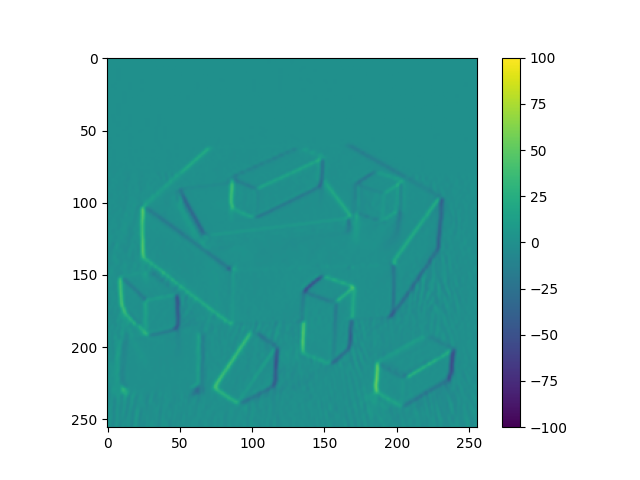
\includegraphics[width=\textwidth]{figures/deriv/ix.png}
         \caption{$I_{x}$}
         \label{fig:I_{x}}
     \end{subfigure}
     \hfill
     \begin{subfigure}[b]{0.3\textwidth}
         \centering
         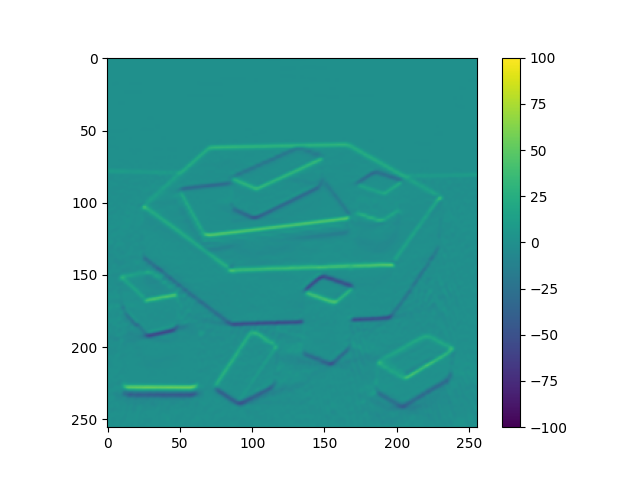
\includegraphics[width=\textwidth]{figures/deriv/iy.png}
         \caption{$I_{y}$}
         \label{fig:I_{y}}
     \end{subfigure}
     \hfill
     \begin{subfigure}[b]{0.3\textwidth}
         \centering
         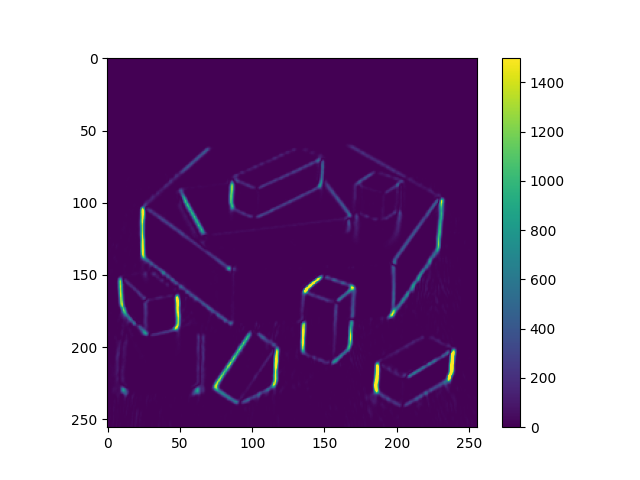
\includegraphics[width=\textwidth]{figures/deriv/ixx.png}
         \caption{$I_{xx}$}
         \label{fig:I_{xx}}
     \end{subfigure}
     \hfill
     \begin{subfigure}[b]{0.3\textwidth}
         \centering
         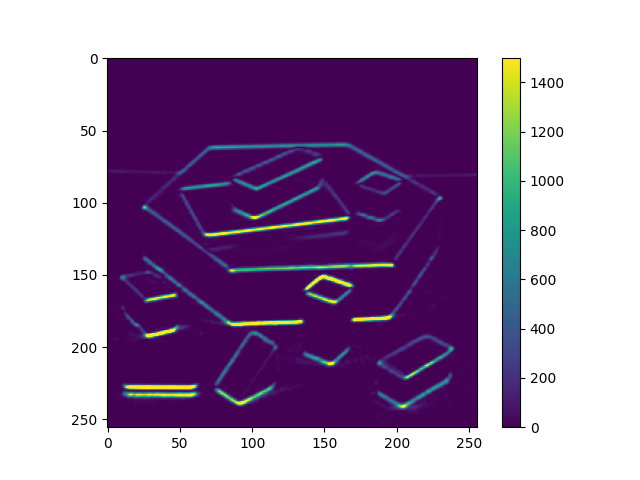
\includegraphics[width=\textwidth]{figures/deriv/iyy.png}
         \caption{$I_{yy}$}
         \label{fig:I_{yy}}
     \end{subfigure}
     \hfill
     \begin{subfigure}[b]{0.3\textwidth}
         \centering
         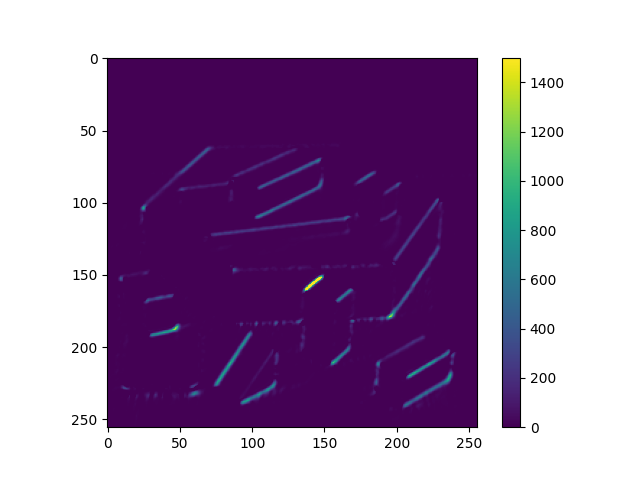
\includegraphics[width=\textwidth]{figures/deriv/ixy.png}
         \caption{$I_{xy}$}
         \label{fig:I_{xy}}
     \end{subfigure}
     \hfill
     \begin{subfigure}[b]{0.3\textwidth}
         \centering
         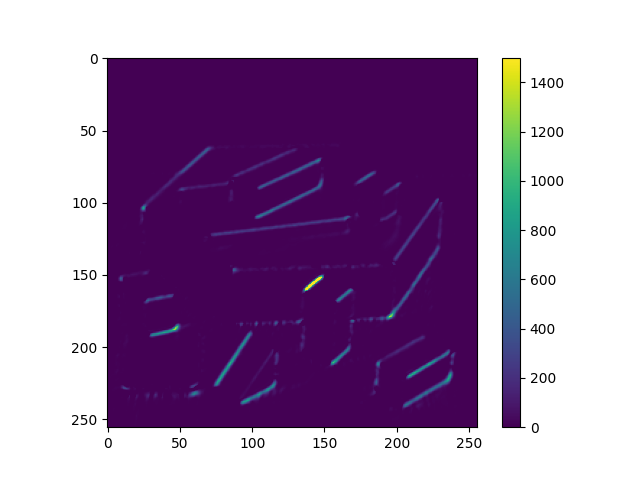
\includegraphics[width=\textwidth]{figures/deriv/ixy.png}
         \caption{$I_{yx}$}
         \label{fig:I_{yx}}
     \end{subfigure}
     
        \caption{Image Derivatives \& Products}
        \label{fig:deriv}
\end{figure}


\begin{figure}[H]
     \centering
     \begin{subfigure}[b]{0.3\textwidth}
         \centering
         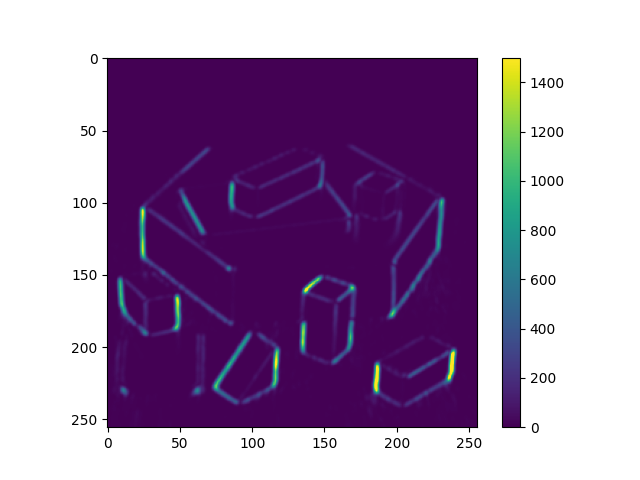
\includegraphics[width=\textwidth]{figures/deriv/ixxs.png}
         \caption{$I_{xxs}$}
         \label{fig:I_{xxs}}
     \end{subfigure}
     \hfill
     \begin{subfigure}[b]{0.3\textwidth}
         \centering
         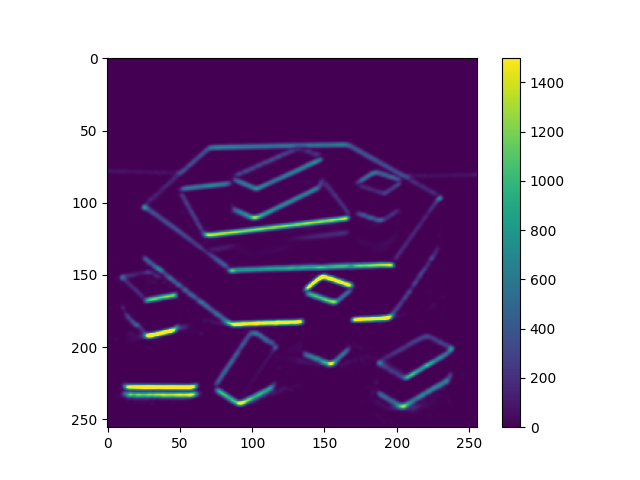
\includegraphics[width=\textwidth]{figures/deriv/iyys.png}
         \caption{$I_{yys}$}
         \label{fig:I_{yys}}
     \end{subfigure}
     \hfill
     \begin{subfigure}[b]{0.3\textwidth}
         \centering
         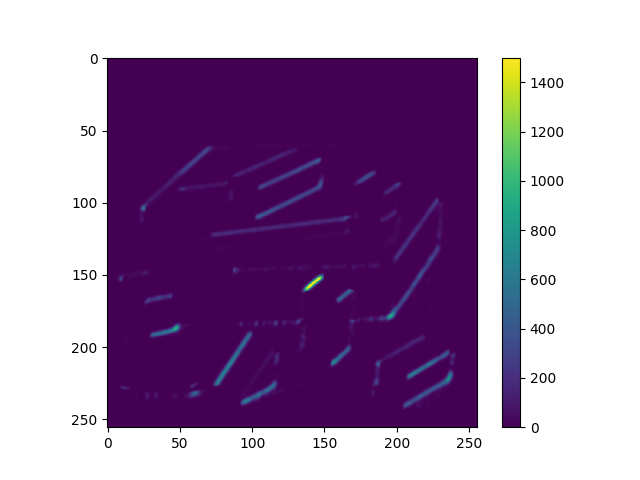
\includegraphics[width=\textwidth]{figures/deriv/ixys.png}
         \caption{$I_{xys}$}
         \label{fig:I_{xys}}
     \end{subfigure}
     
        \caption{Smoothened Derivative Products}
        \label{fig:sdrv}
\end{figure}


\begin{figure}[H]
     \centering
     \begin{subfigure}[b]{0.4\textwidth}
         \centering
         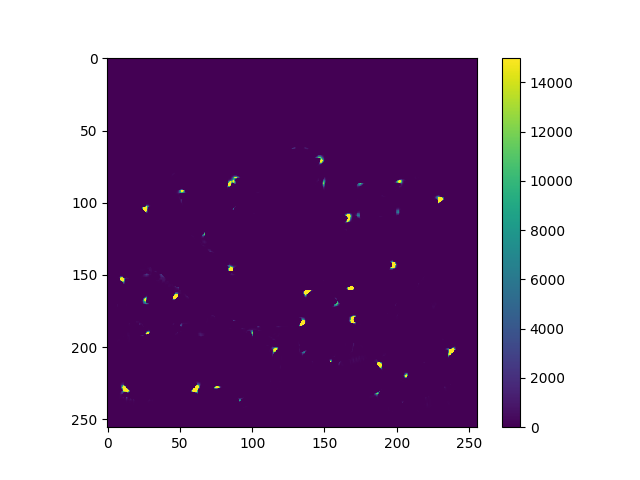
\includegraphics[width=\textwidth]{figures/deriv/R.png}
         \caption{Before Non-Max Sup}
         \label{fig:befharsig}
     \end{subfigure}
     \begin{subfigure}[b]{0.4\textwidth}
         \centering
         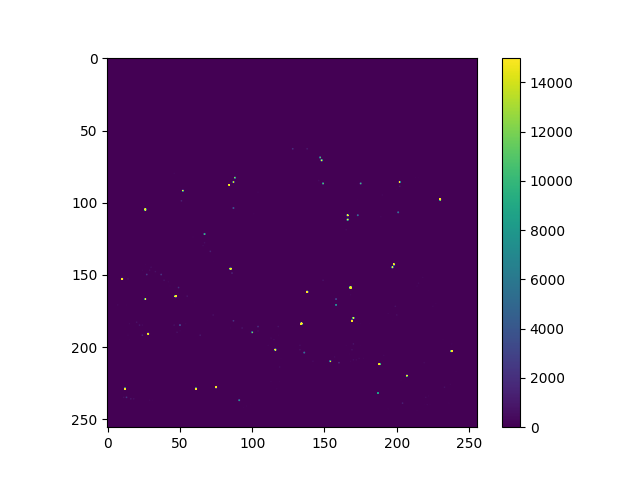
\includegraphics[width=\textwidth]{figures/deriv/RR.png}
         \caption{After Non-Max Sup}
         \label{fig:aftharsig}
     \end{subfigure}
     
        \caption{Harris Corner Signal Value}
        \label{fig:harsig}
\end{figure}


\subsection{Experiments}

    % \begin{figure*}[!h]
    %     \centering
    %     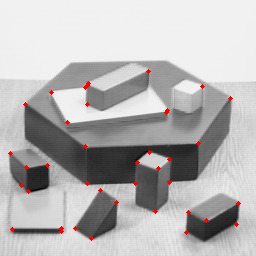
\includegraphics[width=0.3\textwidth]{figures/blocks_harris.png}
    %     \caption{Harris Corner Detection on Blocks}
    %     \label{fig:block_harris}
    % \end{figure*} 

\begin{figure}[!h]
     \begin{subfigure}[b]{0.4\textwidth}
         \centering
         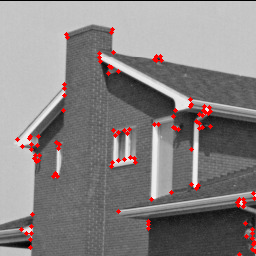
\includegraphics[width=\textwidth]{figures/house_harris.png}
         \caption{$House$}
         \label{fig:house}
     \end{subfigure}
     \hfill
     \begin{subfigure}[b]{0.4\textwidth}
         \centering
         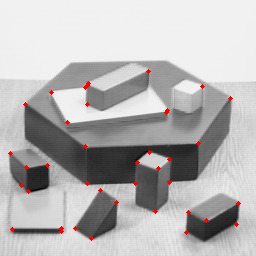
\includegraphics[width=\textwidth]{figures/blocks_harris.png}
         \caption{$Blocks$}
         \label{fig:block}
     \end{subfigure}
        \caption{Harris Corner Detection}
        \label{fig:harr}
\end{figure}
    



\begin{center}
    \raggedright
    I have tested my harris corner implementation on two given images. My algorithm has achieved to detect several keypoints as in Figure \ref{fig:harr}. In Figure \ref{fig:house}, window corners, pipe corners, rectangular corners like chimney and roof are clearly captured by the algorithm. Interestingly one point near the vertical pipe along the edge does not make much sense as it is not a corner but it is most probably due to the high pixel contrast difference between white pipe and dark bricks. In Figure \ref{fig:block}, keypoints are even more obvious and they are all localised with the corners of the geometric prisms except for one outlier on the left rectangle there is a keypoint along the edge which I also believe might be due to high contrast difference between dark object and white ground. Also, I observe some missed keypoints on top of the hexagon as there is lower contrast and background is also low resulting in low corner score signals compared to other parts of the image.
\end{center}



\subsection{Challenges}

\begin{center}
    \raggedright
    During my experiments, I faced some challenges to capture keypoints. The first problem was that I was not able to get any keypoints which happened to be due to too much gaussian convolution. I was applying gaussian convolution both for the image, image gradients, and the squared gradient terms of the matrix which decreased the signal strength due to too much smoothening. Then I applied gaussian convolution to squared gradients term directly and only which kept sufficient signal strength for the detection.
\end{center}
% too much gaussian => less feature points => mitigate signal strength




%%%%%%%%%%%%%%%%%
%   PART-2: Feature Matching   %
%%%%%%%%%%%%%%%%%
% \pagebreak
\section{Feature Matching}


\subsection{Implementation}

\begin{center}
    \raggedright
    In this part, I implemented SSD feature distance function and three different feature matching algorithms for the keypoints. SSD implementation is straightforward: given two feature descriptors of size F1=(q1, d) and F2=(q2, d), we need to calculate (q1, q2) matrix with each cell having squared error difference for each feature vector between $F1_{i}$ and $F2_{j}$. I reshaped my tensors in order to get the right broadcasting in numpy. So I reshaped F1 $=>$ (q1, 1, d) and F2 $=$ (q2, d) (same shape). $F1 - F2$ gives a difference matrix of (q1, q2, d). Then we take the square to calculate squared error for each feature dimension along d. Finally, we sum along feature dimension to get the ssd matrix of dimension (q1, q2) in which each cell denotes the similarity value for each keypoint pair from descriptor-1 (F1) and descriptor-2 (F2).

    For the keypoint matching algorithm, we are asked to implement 3 different ways to match the keypoints: one-way, mutual, and ratio. The matching makes use of the \textbf{ssd} calculation and the (q1, q2) distance matrix. 
    
    One-way nearest neighbor feature matching is based on matching the keypoints of the first image to the nearest keypoints in the second image resulting in (q1,2) matches: q1 many and 2 indices in F1 and F2 correspondingly. In the implementation, I just took argmin accross q2 th channel of (q1,q2) ssd matrix.
    
    Mutual nearest neighbor feature matching is one-way feature matching and another one-way feature matching with the order of images reversed. Then the indices from these 2 one-way feature matches are kept if they are captured from both ways. In the implementation, I applied one-way matching with different order of the descriptors and just selected matches if they exist in both of the ways.

    Ratio based nearest neighbor feature matching is the ratio of one-way best match and one-way second best match that is thresholded by a value ie. if this ratio is smaller than the threshold the match is accepted. This puts a more strict condition for the cases where threshold is between (0,1). In the implementation, I applied one-way match to find the best matches and used np.partition to get second best matches. Then took the ratio and thresholded the matches simply.
    
\end{center}

\subsection{Experiments}

\begin{center}
    \raggedright

    The experiment is conducted on a pair of book image with different slight orientations. Harris corner keypoints are obtained and then a descriptor function fuses information about the keypoint coordinates and harris signal value to a 81-dim feature vector. That is followed by ssd calculation and matching algorithms. Harris keypoint detections in both images are depicted in Figure \ref{fig:harsigbooks}. The matching results areshown in Figure \ref{fig:bookmatch} as expected must be mostly as straight as possible with few exceptions (tilted lines). One-way, mutual, and ratio:0.5 have 428, 332, and 242 feature matches respectively. The matching condition gets more stricter from one-way to ratio matching and as expected we have less matches. Ratio:0.9 is less stricter than ratio:0.5 and have more matches and lines depicted as a result.
    
\end{center}



\begin{figure}[H]
     \centering
     \begin{subfigure}[b]{0.4\textwidth}
         \centering
         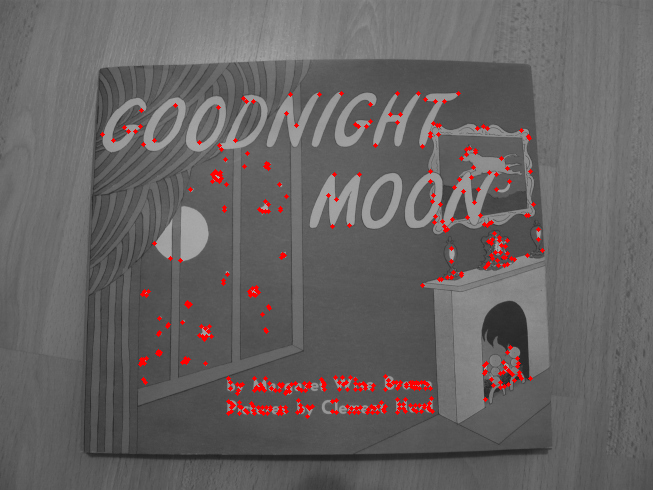
\includegraphics[width=\textwidth]{figures/I1_harris-checkpoint.png}
         \caption{Book IMG-1}
         \label{fig:book1}
     \end{subfigure}
     \begin{subfigure}[b]{0.4\textwidth}
         \centering
         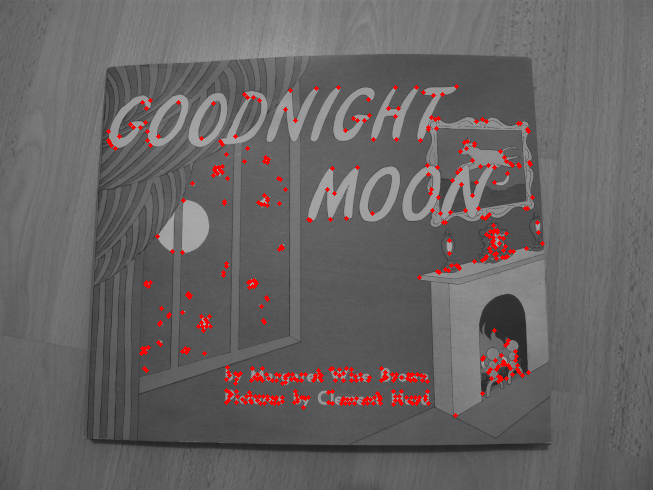
\includegraphics[width=\textwidth]{figures/I2_harris-checkpoint.png}
         \caption{Book IMG-2}
         \label{fig:book2}
     \end{subfigure}
     
        \caption{Harris Corner Detection: Books}
        \label{fig:harsigbooks}
\end{figure}


\begin{figure}[H]
     \centering
     \begin{subfigure}[b]{0.4\textwidth}
         \centering
         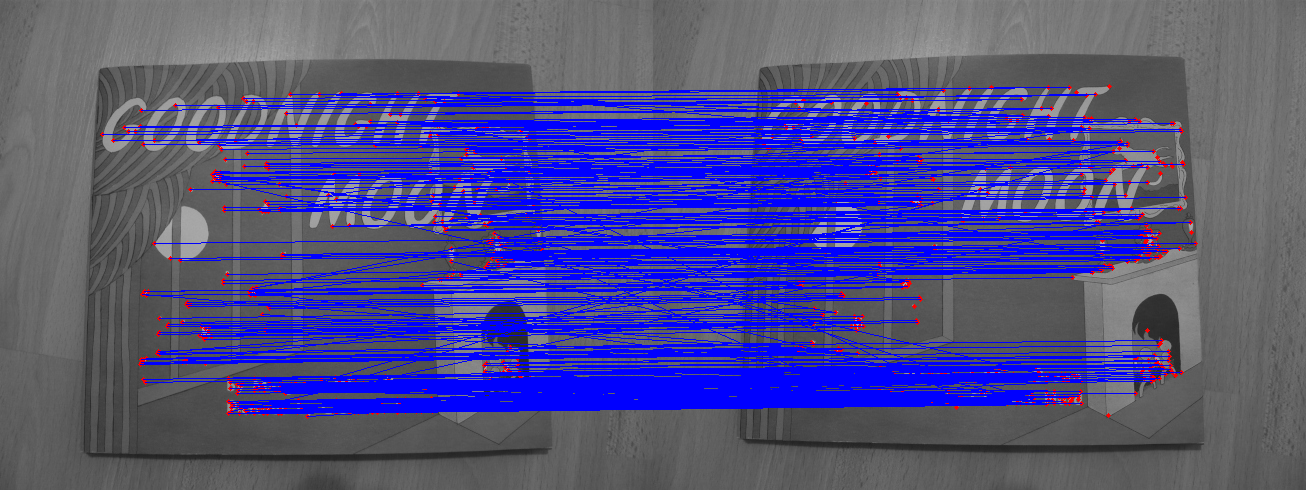
\includegraphics[width=\textwidth]{figures/match_ow.png}
         \caption{One-Way}
         \label{fig:oneway}
     \end{subfigure}
     \begin{subfigure}[b]{0.4\textwidth}
         \centering
         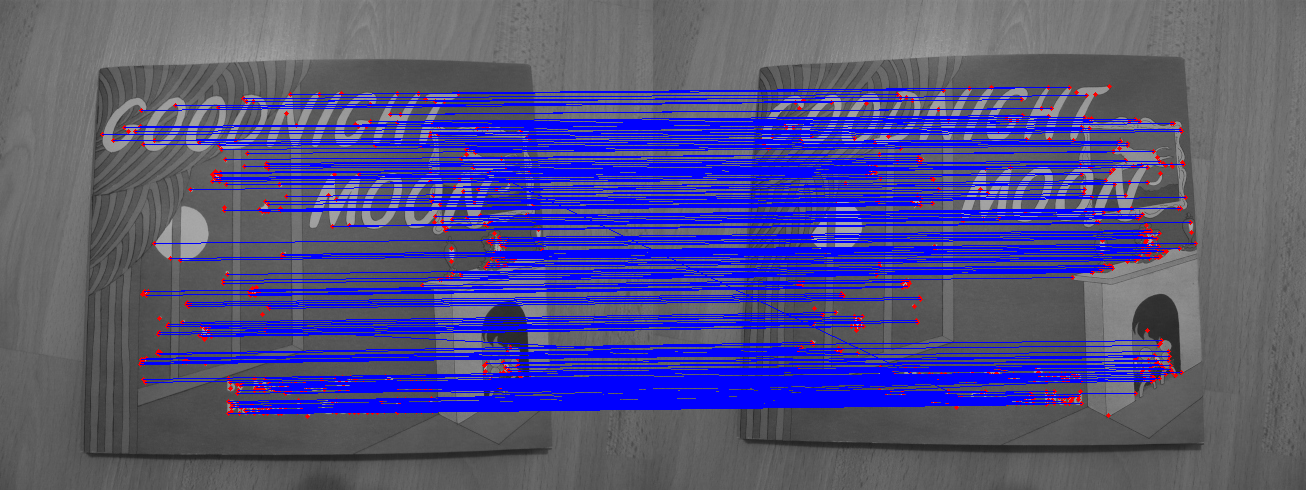
\includegraphics[width=\textwidth]{figures/match_mutual.png}
         \caption{Mutual}
         \label{fig:mutual}
     \end{subfigure}
     \begin{subfigure}[b]{0.4\textwidth}
         \centering
         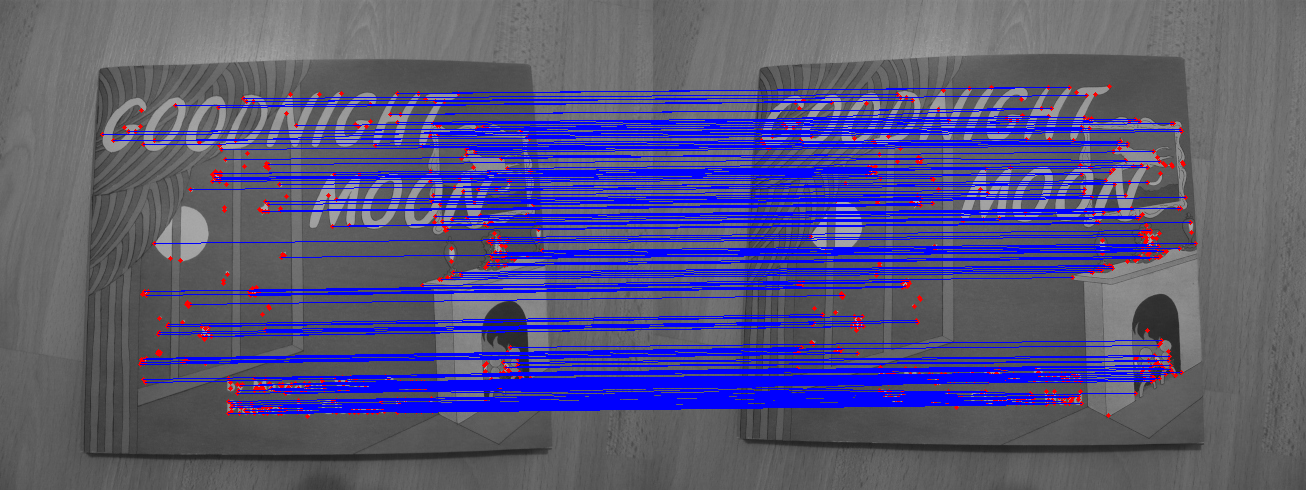
\includegraphics[width=\textwidth]{figures/match_ratio0.5.png}
         \caption{Ratio: 0.5}
         \label{fig:ratio0.5}
     \end{subfigure}
     \begin{subfigure}[b]{0.4\textwidth}
         \centering
         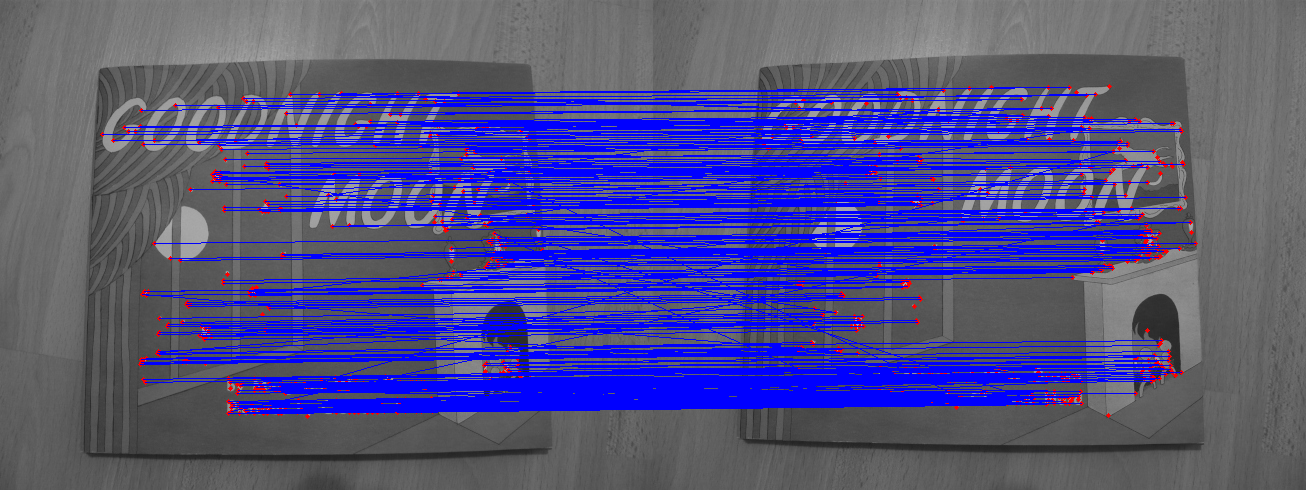
\includegraphics[width=\textwidth]{figures/match_ratio0.9.png}
         \caption{Ratio: 0.9}
         \label{fig:ratio0.9}
     \end{subfigure}     
        \caption{Feature Matching: Books}
        \label{fig:bookmatch}
\end{figure}



\subsection{Challenges}
% broadcasting => 
% ssd calculation => broadcasting problem

\begin{center}
    \raggedright

    I faced some difficulties and bugs during my implementation. The most critical mistake I did was during the reshaping operation of my tensors which I needed for broadcasting to calculate ssd matrix.   
\end{center}


    \begin{minted}[mathescape, linenos]{python}
    diff = desc1.reshape(dw1, 1, dh1) - desc2.reshape(dw2, dh2, 1) # wrong, dimension order violated
    diff = desc1.reshape(dh1, 1, dw1) - desc2 # alternative solution no permutation needed
    \end{minted}

\begin{center}
    \raggedright
    (dw2, dh2, 1) reshaping violates the order in the dimension, it just transforms the dimension without swapping dimensions as we want. So the solution would be with tranpose operation or alternatively without any extra reshaping as illustrated in the code above. With the wrong method I could not match the best pair of keypoints resultin in many cross lines rather than straight.
    
\end{center}
    
\end{document}
